\documentclass[a4paper,11pt]{article}
\usepackage[utf8]{inputenc}
\usepackage[paper=a4paper]{geometry}
\usepackage[numbers]{natbib}
\usepackage{hyperref}
\hypersetup{
    colorlinks=true,
    linkcolor=darkgray,
    filecolor=magenta,
    urlcolor=cyan,
    citecolor=green
    }
\usepackage{multicol}
\usepackage{sectsty}
\usepackage{subfiles}
\usepackage{enumitem}
\usepackage{physics}
\usepackage{pgfplots}
\usepackage{listings}
\usepackage{amsmath}
\usepackage{graphicx}
\usepackage[nottoc,numbib]{tocbibind}
\usepackage[toc,page]{appendix}
\graphicspath{ {./Media} }
\pgfplotsset{width=7cm, compat=1.9}
\newlist{worddefs}{description}{1}
\setlist[worddefs]{font=\bfseries, labelindent=\parindent, leftmargin=6em, style=sameline}
\definecolor{dkgreen}{rgb}{0,0.6,0}
\definecolor{gray}{rgb}{0.5,0.5,0.5}
\definecolor{mauve}{rgb}{0.58,0,0.82}
\lstset{frame=tb, language=C++,
aboveskip=3mm, belowskip=3mm, showstringspaces=false, columns=flexible,
basicstyle={\small\ttfamily}, numbers=none, numberstyle=\tiny\color{gray},
keywordstyle=\color{blue}, commentstyle=\color{dkgreen},
stringstyle=\color{mauve}, breaklines=true, breakatwhitespace=true, tabsize=3 }

%\sectionfont{\fontsize{11}{11}\selectfont}
%\subsectionfont{\fontsize{11}{11}\selectfont}

%opening
\title{\textbf{Simulating Fluid Motion using Smoothed Particle Hydrodynamics}}
\author{Aayush Joshi}
\date{}
\begin{document}
\maketitle
\par\noindent\rule{\textwidth}{0.3pt}

\begin{abstract}
\noindent \textit{This paper covers a method of computational fluid dynamics known as Smoothed Particle Hydrodynamics. Within the introduction, the paper presents the motivations for this project, a brief introduction to SPH and outlines the success crtieria for the artefact. In the research review, the paper provides a history of the SPH techniques as well as alternative CFD approaches considered in industrial applications such as Aerospace. The theoretical model outlines and elaborates on a mathematical brief for each section of SPH and Development shows the implementation of each section of the theoretical model in C++. Development also outlines the added interactive elements using SFML and ImGui. Finally, the evaluation measures the success of the overall project to the criteria outlined within the introduction.}
\end{abstract}

\par\noindent\rule{\textwidth}{0.3pt}
\begin{figure}[h]
\centering
 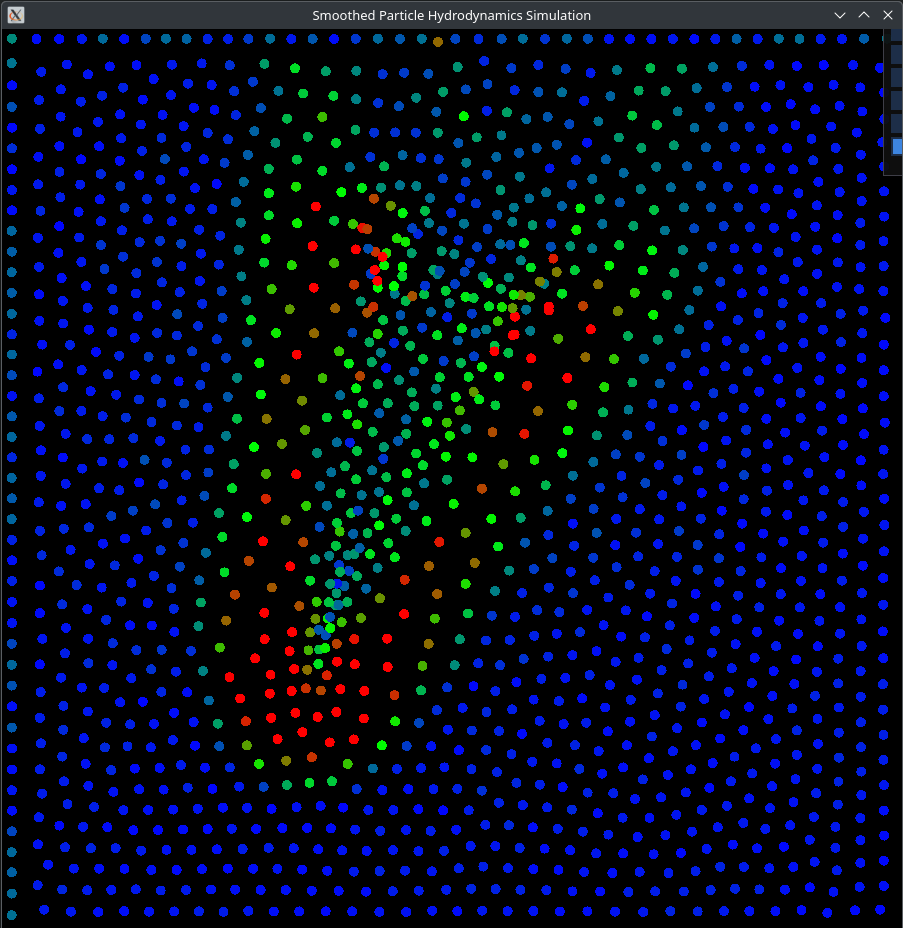
\includegraphics[width=0.5\textwidth]{mouse_drag.png} \par
 Final interactive SPH implementation.
\end{figure}

\newpage
\tableofcontents
\newpage
\begin{multicols}{2}
\subfile{intro.tex}
\pagebreak
\subfile{research_review.tex}
\pagebreak
\subfile{theoretical_model.tex}
\pagebreak
\subfile{development.tex}
\pagebreak
\subfile{evaluation.tex}
\pagebreak

\newpage
\nocite{*}
\bibliography{bibfile.bib}
\end{multicols}
\pagebreak
\subfile{appendix.tex}
\bibliographystyle{IEEEtran}
\end{document}
